
\begin{center}
\begin{tikzpicture}
	\pic[yshift=10mm,rotate=180] (topsurface){frame=2.5cm};
	\node[Bpulley, yshift=-20mm] (pulley1) at (topsurface-center){};
	\node[pulley, xshift=-5mm] (pulley2) [below of=pulley1]{};
	\tzline(pulley1.west)(pulley2.west)
	\tzline(pulley1.center)(pulley2.east)
	\tzline(pulley1.center)(topsurface-center)
	\tzdot*(pulley1.center)
	\tzdot*(pulley2.center)
	\tzline+[->](pulley1.east)(0, -2){$F=20\N$}[b]
	\node[block] (block1) [below of=pulley2]{$2\kg$};
	\tzline(pulley2.center)(block1.north)
\end{tikzpicture}
\end{center}

\begin{center}
\begin{tikzpicture}
\def\ph{0.6}%pulley-height
	\fill[pattern=north east lines](0, 0)--(8, 0)--(8, -3)--(7.75, -3)--(7.75, -0.25)--(0, -0.25)--cycle;
	\draw[thick](0, 0)--(8, 0)--(8, -3);
	\node[pulley] (pulley1) at (4, \ph){};
	\node[pulley] (pulley2) at (8+\ph*cos{45}, \ph){};
	\tzdot*(pulley1.center)
	\node[block, scale=1.25] (block1) at (1, 0.5){$2\kg$};
	\tzline(pulley1.center)(block1.10)
	\tzline(pulley1.south)(pulley2.south)
	
	\tzline(pulley2.center)(8, 0)
	\tzdot*(pulley2.center)
	\node[block, scale=1.25] (block2) at (8+\ph*cos{45}+0.5, -2){$1\kg$};
	\tzline(pulley2.east)(block2.north)
	\tzline(pulley1.north)(pulley2.north)
\end{tikzpicture}
\end{center}



\begin{center}
\begin{tikzpicture}
	\pic[yshift=1cm, rotate=180](hinge) {frame=2cm};
	\node[pulley] (pulley1) at (0, 0){};
	\tzline(hinge-center)(pulley1.center)
	\tzdot*(pulley1.center)
	\node[block] (block1)[below of=pulley1, xshift=-5mm]{$4\kg$};
	\node[block] (block2)[below of=pulley1, xshift=5mm, yshift=-10mm]{$6\kg$};
	\tzline(pulley1.west)(block1.north)
	\tzline(pulley1.east)(block2.north)
\end{tikzpicture}
\end{center}



\begin{center}
\begin{tikzpicture}
	\pic {frame=5cm};
	\node[block] (block1) at (0, 0.4){$2\kg$};
	\node[block] (block2) [above of=block1, yshift=-1cm]{$1\kg$};
\end{tikzpicture}
\end{center}




\begin{center}
\begin{tikzpicture}
\pic[yshift=1cm, rotate=180](hinge) {frame=2cm};
	\node[lpulley] (pulley1) at (0, 0){};
	\node[pulley] (pulley2)[below of=pulley1, xshift=6mm]{};
	\node[block] (block1)[below of=pulley1, xshift=-6mm]{$1$};
	\node[block] (block2)[below of=pulley2, xshift=-5mm]{$2$};
	\node[block] (block3)[below of=pulley2, xshift=5mm]{$3$};
	\tzline(hinge-center)(pulley1.center)
	\tzdot*(pulley1.center)
	\tzdot*(pulley2.center)
	
	\tzline(pulley1.west)(block1.north)
	\tzline(pulley1.east)(pulley2.center)
	\tzline(pulley2.west)(block2.north)
	\tzline(pulley2.east)(block3.north)
\end{tikzpicture}
\end{center}


\begin{center}
\begin{tikzpicture}
\pic[yshift=1cm, rotate=180](hinge) {frame=2cm};
	\node[lpulley] (pulley1) at (0, 0){};
	\node[pulley] (pulley2)[below of=pulley1, xshift=6mm]{};
	\node[block] (block1)[below of=pulley1, xshift=-6mm]{$1$};
	\node[block] (block2)[below of=pulley2, xshift=-5mm]{$2$};
	\node[block] (block3)[below of=pulley2, xshift=5mm]{$3$};
	\tzline(hinge-center)(pulley1.center)
	\tzdot*(pulley1.center)
	\tzdot*(pulley2.center)
	
	\tzline(pulley1.west)(block1.north)
	\tzline(pulley1.east)(pulley2.center)
	\tzline(pulley2.west)(block2.north)
	\tzline(pulley2.east)(block3.north)
\end{tikzpicture}
\end{center}


\begin{center}
\begin{tikzpicture}
	\fill[pattern=north east lines](0, 0)--(8, 0)--(8, -3)--(7.75, -3)--(7.75, -0.25)--(0, -0.25)--cycle;
	\draw[thick](0, 0)--(8, 0)--(8, -3);
	\node[pulley] (pulley1) at (1.5, 0.9){};
	\tzline+(pulley1.center)(0, -0.9)
	\tzdot*(pulley1.center)
	\node[block] (block1) at (4, 0.4){$1\kg$};
	\tzline(pulley1.south)(block1.west)
	\node[block] (block3) [right of=block1]{$3\kg$};
	\tzline(block1.east)(block3.west);
	
	\node[pulley] (pulley2) at (8+0.9*cos{45}, 0.9){};
	\tzline(pulley2.center)(8, 0)
	\tzdot*(pulley2.center)
	\node[block] (block2) at (8+0.9*cos{45}+0.5, -2){$2\kg$};
	\tzline(pulley2.east)(block2.north)
	\tzline(pulley1.north)(pulley2.north)
\end{tikzpicture}
\end{center}



\begin{center}
\begin{tikzpicture}
\node[block] (block1) at (0, 0){$1\kg$};
\tzline+[->](block1.north)(0, 1)
\end{tikzpicture}
\end{center}




\begin{center}
\begin{tikzpicture}
	\fill[pattern=north east lines](0, 0)--(8, 0)--(8, -3)--(7.75, -3)--(7.75, -0.25)--(0, -0.25)--cycle;
	\draw[thick](0, 0)--(8, 0)--(8, -3);
	\node[pulley] (pulley1) at (2, 0.9){};
	\tzline+(pulley1.center)(0, -0.9)
	\tzdot*(pulley1.center)
	\node[block] (block1) at (4.5, 0.4){$M$};
	\tzline(pulley1.south)(block1.west)
	
	\node[pulley] (pulley2) at (8+0.9*cos{45}, 0.9){};
	\tzline(pulley2.center)(8, 0)
	\tzdot*(pulley2.center)
	\node[block] (block2) at (8+0.9*cos{45}+0.5, -2){$M$};
	\tzline(pulley2.east)(block2.north)
	\tzline(pulley1.north)(pulley2.north)
\end{tikzpicture}
\end{center}


\begin{center}
\begin{tikzpicture}
	\pic {frame=5cm};
	\node[block] (block1) at (0, 0.4){$2\kg$};
	\node[block] (block2) [above of=block1, yshift=-1cm]{$1\kg$};
\end{tikzpicture}
\end{center}


\begin{center}
\begin{tikzpicture}
	\pic[xshift=1cm] (0, 0) {frame=8cm};
	\tzcoors(0, 0)(A)(3, 0)(B)(0,3)(C);
	\tzpolygon(A)(B)(C);
	\tzanglemark(C)(B)(A){$30^\circ$}(15pt)
	\node[block, yshift=4mm, rotate around={-45:(B)}] (box1) at (0, 0) {$2\kg$};
	\node[block, rotate=-45] (box2) [right of=box1, xshift=-9.7mm]{$4\kg$};
\end{tikzpicture}
\end{center}



\begin{center}
\begin{tikzpicture}
\tzcoor(0, 0)(O)
	\pic[yshift=10mm,rotate=180] (hinge){frame=2cm};
	\node[pulley] (pulley1) at (O){};
	\node[block] (box1) [below of=pulley1, xshift=-5mm] {$1\kg$};
	\node[block] (box2) [below of=pulley1, xshift=5mm, yshift=-5mm] {$2\kg$};
	\tzdot*(pulley1.center)
	\tzline(hinge-center)(pulley1.center)
	\tzline(pulley1.west)(box1.north)
	\tzline(pulley1.east)(box2.north)
	\tzline+[->](box1.south)(0, -1){$F$}[b]
\end{tikzpicture}
\end{center} 



\begin{center}
\begin{tikzpicture}
\tzcoor(0, 0)(O)
	\pic[yshift=-4.3mm] at (O) {frame=6cm};
	\node[block] (box1) at (O) {$4\kg$};
	\node[block] (box2) [right of=box1, xshift=-9.7mm] {$2\kg$};
	\tzline+[<-](box1.west)(-1.5, 0){$20\N$}[midway, a]
\end{tikzpicture}
\end{center} 


\begin{center}
\begin{tikzpicture}
\tzcoor(0, 0)(O)
	\pic[yshift=-4.3mm, xshift=5mm] at (O) {frame=7cm};
	\node[block] (box1) at (O) {$3\kg$};
	\node[block] (box2) [right of=box1, xshift=-9.7mm] {$2\kg$};
	\node[block] (box3) [right of=box2, xshift=-9.7mm] {$1\kg$};
	\tzline+[<-](box1.west)(-1.5, 0){$12\N$}[midway, a]
\end{tikzpicture}
\end{center} 



\begin{center}
\begin{tikzpicture}
\pic (surface) {frame=9cm};
	\node[block, yshift=4mm] (block1) at (surface-center){$12\kg$};
	\node[block] (block2) [right of=block1]{$15\kg$};
	\node[block] (block3) [left of=block1]{$3\kg$};
	\tzline(block3.east)(block1.west){$T_1$}[midway, a]
	\tzline(block1.east)(block2.west){$T_2$}[midway, a]
	\tzline[->]"force"(block2.east)([turn]30:2)
	\tzvXpointat{force}{3}(A)
	%\tzdot*(A)
	\tzline+[dashed]"dashedline"(block2.east)(2, 0)
	\tzvXpointat{dashedline}{3}(B)
	%\tzdot*(B)
	\tzanglemark(B)(block2.east)(A){$30^\circ$}(16pt)
\end{tikzpicture}
\end{center}	


\begin{center}
\begin{tikzpicture}
\tzcoor(0, 0)(O)
	\pic[yshift=10mm,rotate=180] (hinge){frame=2.5cm};
	\node[pulley] (pulley1) at (O){};
	\node[block] (box1) [below of=pulley1, xshift=-5mm] {$4\kg$};
	\node[block] (box2) [below of=pulley1, xshift=5mm, yshift=-5mm] {$3\kg$};
	\node[block] (box3) [below of=box2]{$1\kg$};
	\tzline(box2.south)(box3.north)
	\tzdot*(pulley1.center)
	\tzline(hinge-center)(pulley1.center)
	\tzline(pulley1.west)(box1.north)
	\tzline(pulley1.east)(box2.north)
\end{tikzpicture}
\end{center} 


\begin{center}
\begin{tikzpicture}
	\pic[yshift=10mm,rotate=180] (topsurface){frame=4cm};
	\node[pulley, yshift=-15mm] (pulley1) at (topsurface-center){};
	\node[pulley, xshift=5mm] (pulley2) [below of=pulley1] {};
	\node[pulley, xshift=5mm] (pulley3) [below of=pulley2] {};
	\node[block, xshift=5mm] (block1) [below of=pulley3] {$2$};
	\tzline(topsurface-center)(pulley1.center)
	\tzdots*(pulley1.center) (pulley2.center) (pulley3.center);
	\tzline(pulley1.east)(pulley2.center)
	\tzline(pulley2.east)(pulley3.center)
	\tzline(pulley3.east)(block1.north)
	\node[plank, yshift=-50mm] (plank1)[below of=pulley1]{$1$};
	\tzline+(pulley1.west)(0, -5 - 1.4)
	\tzline+(pulley2.west)(0, -5 + 0.4)
	\tzline+(pulley3.west)(0, -5 + 2.2)
\end{tikzpicture}
\end{center}



	
\begin{center}
\begin{tikzpicture}
\node[lift] (lift) at (0, 0){};
\node[Hblock, yshift=6 mm] (block1) at (lift.south){$5\kg$};
\node[hblock, yshift=6 mm] (block2) at (block1.north){$2\kg$};
\tzline+[->](3.5, -2.5)(0, 3){$5\mpss$}[a]
\end{tikzpicture}
\end{center}

	
\begin{center}
\begin{tikzpicture}
\tzcoor(0, 0)(O)
	\pic[yshift=10mm,rotate=180] (hinge){frame=3cm};
	\node[pulley] (pulley1) at (O){};
	\node[block] (box1) [below of=pulley1, xshift=-5mm] {$A$};
	\node[pulley, xshift=5mm, yshift=-10mm] (pulley2) [below of=pulley1]{};
	\node[block] (box2) [below of=pulley2, xshift=5mm] {$C$};
	\node[block] (box3) [below of=pulley2, xshift=-5mm, yshift=-5mm]{$B$};
	\tzline(pulley2.west)(box3.north)
	\tzline(pulley2.east)(box2.north)
	\tzdot*(pulley1.center)
	\tzline(hinge-center)(pulley1.center)
	\tzline(pulley1.west)(box1.north)
	\tzline(pulley1.east)(pulley2.center)
	\tzdot*(pulley2.center)
\end{tikzpicture}
\end{center} 


            
 
    \begin{center}
        \begin{tikzpicture}[scale=2]
            \coordinate (A) at (0.707, 0.707);
            \coordinate (B) at (-0.707, 0.707);
        
            \tzarc (0, 0)(135:405:1)
            \tzarc (0, 0)(45:135:0.2)
            \tzdot*(A)
            \tzarc[->](0, 0)(45:135:1)
            \tzlines*[dashed](B)(0, 0){$R$}[black, r](A);
            \node at (A)[above=2mm]{$A$};
            \node at (B)[above=2mm]{$B$};
            \node at (0,0)[above=5mm]{$\dfrac{\pi}{2}$};
        \end{tikzpicture}
    \end{center}

    \begin{center}
        \begin{tikzpicture}[cap=round, scale=0.6]
            %\tzaxes[->](-1, -1)(5, 5)
            \draw[->] (-1, 0)--(5, 0)node[right]{$t$};
            \draw[->] (0, -2)--(0, 4)node[left]{$v$};
            \draw (0, -1)--(4, 3);
            \node at (1, 0) [below]{$1$};
            \node at (3, 0) [below]{$3$};
            \draw[dashed] (3, 0)--(3, 2);
            \draw[dashed] (0, 2)node[left]{$2$}--(3, 2);
        \end{tikzpicture}
    \end{center}




\begin{center}
\begin{tikzpicture}[scale=0.7]
	\tzaxes(-1, -2.5)(4.5, 3.5){$t(\s)$}{$a(\mpss)$} 
	\tzLFn(0,-2)(1, 0)[0:2.5]
	\tzticks{1}{-2}
\end{tikzpicture}
\end{center}
